\section{\texorpdfstring{Konečné/Afinní projektivní roviny}{Konečné/Afinní projektivní roviny}}
\vspace{5mm}
\large

\begin{definition}[Množinový systém]
    Nechť $X, I$ jsou množiny. Pak
    \[ \M=(M_i)_{i\in I}, \forall i\in I: M_i\subseteq X \]
    nazveme množinovým systémem.

    Kromě množinového zápisu a \emph{Vennova diagramu} také můžeme incidenci značit incidenční maticí $A_{\M}\in\{0,1\}^{X\times I}$, kde $A_{x,i}=1$, právě když $x\in M_i$.
    Alternativou je také bipartitní graf incidence, který definujeme jako
    \[B_{\M}=(X\cup I, \{\{x,i\}: x\in M_i\}) \]
\end{definition}
\begin{definition}[Konečná projektivní rovina]\label{kpr_a}
    Konečná projektivní rovina (KPR) je množinový systém $\mathcal{P}=(X,\LP)$ splňující následující axiomy:
    \begin{itemize}
        \item[(A1)] Pro každé dvě různé množiny $A,B\in\LP$ platí $|A\cap B|=1$
        \item[(A2)] Pro každé dva různé prvky $x,y\in X$ existuje $A\in\LP$ taková, že $x,y\in A$
        \item[(A3)] V $X$ existují čtyři prvky tak, že žádné tři z nich nepatří do stejné množiny z $\LP$.
    \end{itemize}

    Je zvykem prvkům množiny $X$ říkat body a množinám z $\LP$ přímky.
\end{definition}
\begin{note}[Každé dva body v KPR sdílejí právě jednu přímku]
    Pokud $\mathcal{P}=(X,\LP)$ splňuje A1 a A2, pak každé dva různé body $x,y\in X$ náležejí právě jedné společné přímce.
\end{note}
\begin{proof}
    Mějme $x,y\in X$ různé.
    Z A2 máme, že existuje alespoň jedna $A\in\LP$ taková, že $x,y\in A$.
    Pro spor předpokládejme, že existuje i odlišná $B\in\LP$ taková, že $x,y\in B$.
    Pak přímky $A$ a $B$ nesplňují A1, neboť $A\cap B\supset \{x,y\}$, a tedy $|A\cap B|\geq 2$, což je spor.
\end{proof}
\begin{note}[O ekvivalentním axiomu ke čtveřici v KPR]
    Pokud systém $\mathcal{P}=(X,\LP)$ splňuje A1 a A2, pak A3 je ekvivalentní axiomu
    \begin{itemize}
        \item[(A3')] Body systému $\mathcal{P}$ nemohou být pokryty jednou nebo dvěma přímkami z $\LP$.
    \end{itemize}
\end{note}
\begin{proof}
    TODO
\end{proof}
\begin{theorem}[O řádu KPR]
    Pro každou KPR $\mathcal{P}=(X,\LP)$ existuje přirozené číslo $m$ takové, že
    \begin{itemize}
        \item $\forall A\in\LP: |A|=m+1$
        \item $\forall x\in X: |\{A\in\LP: x\in A\}|=m+1$
        \item $|X|=|\LP|=m^2+m+1$
    \end{itemize}

    Toto číslo $m$ nazýváme \textbf{řádem roviny} $\mathcal{P}$ a můžeme psát KPR($m$) pro konečnou projektivní rovinu řádu $m$.
\end{theorem}
\begin{proof}
	Vezmeme $x \notin A \in \LP$.
	Definujme zobrazení které přiřazuje bod z přímky $L$ bod na $A$:
	\[ \varphi:\{ L: x \in L \in \LP \} \to A \]
	Neboli $\varphi(L)$ je průsečík s přímkou A (právě jeden společný bod).
	Různým přímkám přiřadí různé body.
	Nechť sporem existují 2 přímky kterým $\varphi$ přiřadilo stejný bod, pak mají alespoň 2 společné body. Spor s axiomem A1 \cref{kpr_a}.
	Proto $\varphi$ je prosté.

	% 1 predn 14:20
	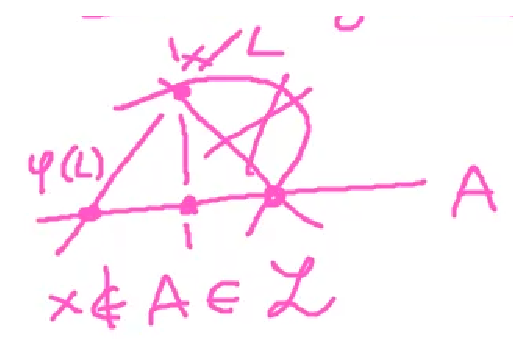
\includegraphics[scale=0.5]{kpr_0.eps}

	Na druhou stranu, každý bod A protíná ještě nějaká přímka $\Rightarrow \varphi$ je na.
	Neboli $\varphi$ je bijekce.

	Vezmeme 2 přímky $A, B$. Dle A3 nemůže pokrývat celou KPR.
	\[ \exists y: y \notin A \land y \notin B \]
	Jelikož $\varphi$ je bijekce
	\[ |A| = \text{\# přímek procházejících}\ y = |B| \]
	Dohromady
	\[ \exists m: \forall A \in \LP: |A| = m + 1 \]

	Nechť $A \in \LP$ libovolná přímka, má $(m + 1)$ bodů.
	Dal bodem $v \in A$ prochází dalších $m$ přímek, pro nichž $v$ je jediným společným bodem, ostatní jsou různé.
	Nazveme je vodorovné.
	Každá z nich má dalších $(m + 1) - 1 = m$ bodů, dohromady $m^2$.
	Vezmeme další bod $s \in A$. Tím prochází dalších $m$ přímek a musí protínat vodorovné právě v 1 bodě.
	Říkáme jim svislé.
	Z ostatních bodů A taky vychází svazek $m$ přímek, další body již ale nejsou.

	Tedy celkem $|X|=|\LP|=m^2+m+1$ bodů a $|\LP| = 1 + m(m +1)$ přímek.

	% todo 1 predn 20:10
	Kanonický obrázek KPR:

	"Přímky" se nerovnají geometrickým přímkám, jen mnemonický název.
\end{proof}
\begin{theorem}[Existence KPR]
    Je-li $m=p^r$ mocnina prvočísla, pak existuje KPR($m$).
\end{theorem}
\begin{proof}
	Konstruktivně pomoci $\mod$ aritmetiky.
	Z algebry $\exists GF(m)$ napíšeme jako
	\[ \{ 1, \ldots, m = 0 \} \]

	Nechť $A = \{ a_0, \ldots, a_{m - 1} \}$ je přímka.
	Označme svazek přímek vycházející z bodu $a_k$:
	\begin{equation}\label{kpr_svaz}
		\forall k \in \{ 0, \ldots, m - 1 \}, \forall b \in [m]: l_{k, b} = \{ a_k \} \cup \{ x_{i, k\cdot i + b}: i \in [m] \}
	\end{equation}
	kde $x_{i, j}$ je bod se souřadnice $(i, j)$ v šachovnice.

	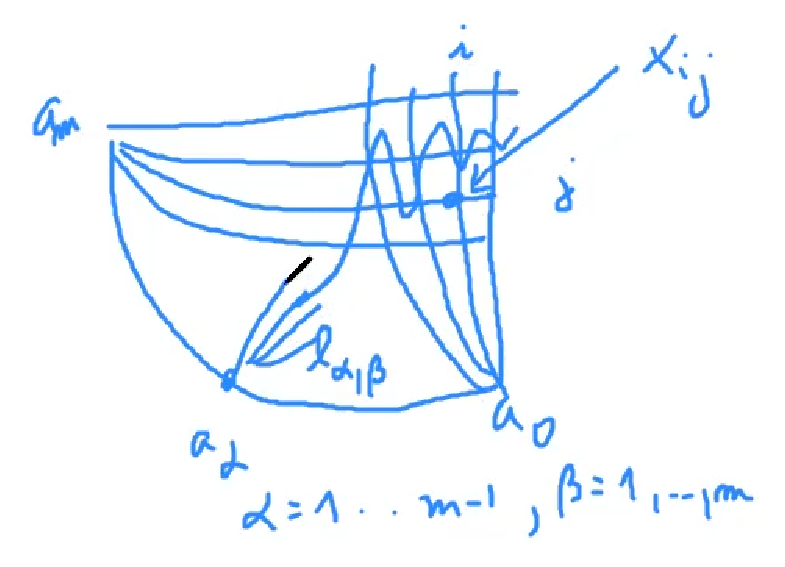
\includegraphics[scale=0.5]{kpr_1.eps}

	Šikmé přímky taky lze vyjádřit pomoci vzorečku \eqref{kpr_svaz}:
	\[ \forall b \in [m]: l_{m, b} = \{ a_m \} \cup \{ x_{i, m\cdot i + b = b}: i \in [m] \} \]

	Ověříme axiomy \cref{kpr_a}:
    	\begin{itemize}
    	    \item[(A1)] Rozborem případů:
		    \begin{enumerate}
			    \item přímky ze stejného svazku dle jednoznačnosti aritmetiky modulo v tělese mají společný prvek pouze $a_k$.
			    \item Stejně pro šikmé přímky, protože je lze stejně vyjádřit.
			    \item Jednobodový průnik přímek ze svazku a vodorovných zaručuje jednoznačný bod $x_{i, j}$.
			    \item Potřebujeme ukázat
				    \[ \forall k_1 \ne k_2, \forall b_1, b_2: |l_{k_1, b_1}, l_{k_2, b_2}| = 1 \]
				    Dle definice přímek ze svazku bod v průniku má souřadnice:
				    \[ x_{i, j} = x_{i, k_1 \cdot i + b_1} = x_{i, k_2 \cdot i + b_2} \Rightarrow k_1 \cdot i + b_1 = k_2 \cdot i + b_2 \iff i = (b_1 - b_2) \cdot (k_2 - k_1)^{-1} \]
				    Z vlastnosti konečného tělesa, takové $i$ je jednoznačné.
		    \end{enumerate}
    	    \item[(A2)] Není potřeba ukazovat rozborem případu. Stačí sečíst dvěma způsoby
		    \[ C = |\{ ((x, y), A) : x, y \in A, x \ne y, A \in \LP \}| \]
		    máme $(m + 1)$ přímek a $\binom{m + 1}{2}$ způsobů zvolit body.
		    Taky ale z A1 2 body spojuje nejvýše 1 přímka, proto $\binom{m^2 + m + 1}{2} \geq C$
		    Dohromady
		    \[ \binom{m^2 + m + 1}{2} = (m^2 + m + 1) m (m + 1) \geq C = (m + 1) \cdot \binom{m + 1}{2} = (m^2 + m + 1) m (m + 1) \]
		    Z rovnosti usoudíme, že každé dvojice odpovídá právě jedna přímka.
    	    \item[(A3)] TODO z konstrukce?
    	\end{itemize}
\end{proof}
\begin{conj}
    KPR($m$) existuje, právě když $m$ je mocnina prvočísla
\end{conj}
\begin{theorem}[KPR(6), Dk později]
    KPR(6) neexistuje.
\end{theorem}
\begin{note}
    KPR(10) neexistuje, ale jediný známý důkaz je počítačovým rozborem případů.

    Neznáme žádnou KPR s řádem rozdílným od mocniny prvočísla.
    Zároveň však známe nekonečně mnoho $m$ takových, že KPR($m$) neexistuje.
    Nejmenší otevřený případ je $m=12$.
\end{note}
\begin{definition}[Konečná afinní rovina]
    Konečná afinní rovina (KAR) je množinový systém $\mathcal{P}=(X,\LP)$ splňující následující axiomy:
    \begin{itemize}
        \item[(AF1)] Pro každé dva různé prvky $x,y\in X$ existuje právě jedna množina $A\in\LP$ taková, že $x,y\in A$
        \item[(AF2)] Pro každou množinu $A\in\LP$ a každý prvek $x\in X$ nenáležící do $A$ existuje právě jedna množina $B\in\LP$ taková, že $x\in B$ a $A\cap B=\emptyset$
        \item[(AF3)] V $X$ existují tři prvky, které nepatří do stejné množiny z $\LP$
    \end{itemize}

    Prvkům množiny $X$ říkáme body, množinám z $\LP$ říkáme přímky, dvě množiny s prázdným průnikem jsou rovnoběžky a dvě množiny s neprázdným průnikem jsou různoběžky.
\end{definition}
\begin{note}[O relaci rovnoběžnosti a směrech]
    Rovnoběžnost přímek v KAR je tranzitivní a symetrická relace na $\LP$.
    Její reflexivní zúplnění je tedy ekvivalence a $\LP$ se tedy rozpadá na několik tříd ekvivalence. Těmto třídám říkáme směry.
    Přímky různých směrů jsou různoběžné.
\end{note}
Q: co když přímky husté?

Q: co když slepíme směry dle ekvivalence?\\
A: Jak slepit? Neporuší to axiomy?

Q: souvisí KAR s hyperbolickou geometrii Lobačevského?\\
A: ano, ale nevíme co dříve.

\begin{theorem}[O řádu KAR]
    Pro každou KAR $\mathcal{P}=(X,\LP)$ existuje $m\in\N$ (nazývané řád roviny $\mathcal{P}$) takové, že:
    \begin{itemize}
        \item $\forall a\in\LP: |A| = m$
        \item $\forall x\in X: |\{A\in\LP: x\in A\}|=m+1$
        \item $|X|=m^2$
        \item $|\LP| = m^2+m$
        \item počet směrů přímek je $m+1$, přičemž každý směr obsahuje $m$ rovnoběžných přímek
    \end{itemize}
\end{theorem}
\begin{proof}
	Vezmeme $x \notin A \in \LP$.
	Definujme zobrazení které přiřazuje bod z přímky $L$ bod na $A$:
	\[ \varphi(L) = L \cap A, \varphi:\{ L: x \in L \in \LP, L \nparallel A \} \to A \]
	Z AF1 $\varphi$ je prosté a je definované pro všechny body A proto $\varphi$ je na $\Rightarrow$ bijekce.

	Jelikož $\varphi$ je bijekce a z AF2 existuje právě 1 rovnoběžka k A procházející bodem $x$:
	\begin{equation}\label{kar_x}
		|A| + 1 = \text{\# přímek obsahujících}\ x
	\end{equation}
	Vezmeme 2 přímky $A, B: A \nparallel B$. Dle AF1, AF2, AF3 $\Rightarrow$ nejde pokryt 2ma různoběžnými přímkami.
	Pak $\exists t \notin A \cup B$, zobrazeni $\varphi$ určuje přímku pro každý bod A, B.
	Neboli $|A| = |B|$.

	Vezmeme 2 rovnoběžky $A, B$ a různoběžku $C$ z předchozího případu usoudíme $|A| = |C| = |B|$.

	Dohromady $\exists m, \forall A \in \LP: |A| = m$.
	Taky z \eqref{kar_x}:
	\[ | \{L : x \in L \in \LP\} | = m + 1 \]

	% 1 predn 58:00
	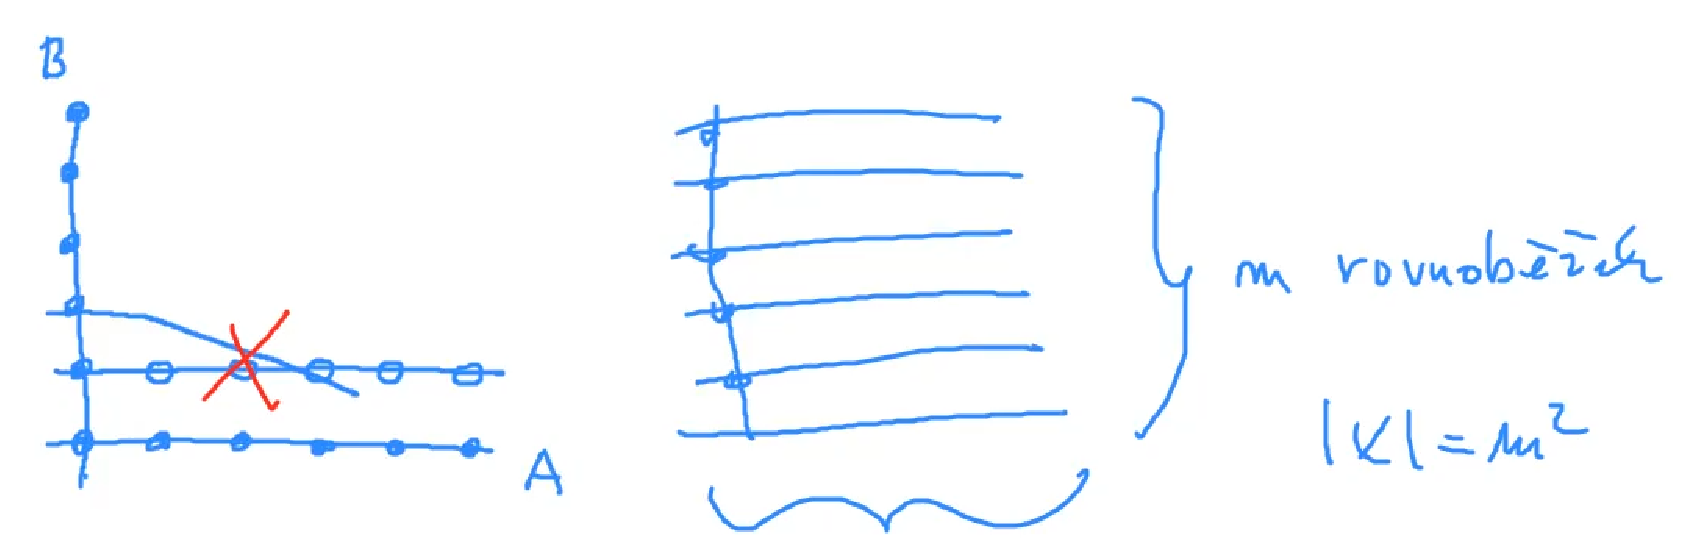
\includegraphics[scale=0.5]{kar_0.eps}

	Vezmeme libovolnou přímku $A$, má $m$ bodů. Přes libovolný bod $a \in A$ prochází další přímka $B$.
	Dle AF2 najdeme ke každému bodu $b_i \in B$ rovnoběžku k $A$ která má dalších $(m - 1)$ bodů.
	Konstrukce dává $m$ rovnoběžek a $m^2$ bodů.
	Dohromady $|X| = m^2$.

	Na jedné straně, počet bodu je $m^2$. Každým bodem prochází $(m + 1)$ přímek.
	Na druhé straně se to rovná počtu přímek krát počet bodů na přímce $m$.
	\[ m^2 \cdot (m + 1) = |\LP| \cdot |A| = |\LP| \cdot m \Rightarrow |\LP| = m \cdot (m + 1) \]

\end{proof}
\begin{consequence}[O vztahu KAR a KPR]
    Každá afinní rovina řádu $m$ vznikne z projektivní roviny řádu $m$ vynecháním jedné přímky a jejích bodů.
    Naopak každá projektivní rovina řádku $m$ vznikne z nějaké afinní roviny řádu $m$ přidáním $m+1$ bodů, každý z nich do všech přímek jednoho směru, a jedné přímky obsahující tyto přidané body.

	% 1 predn 01:03:30
	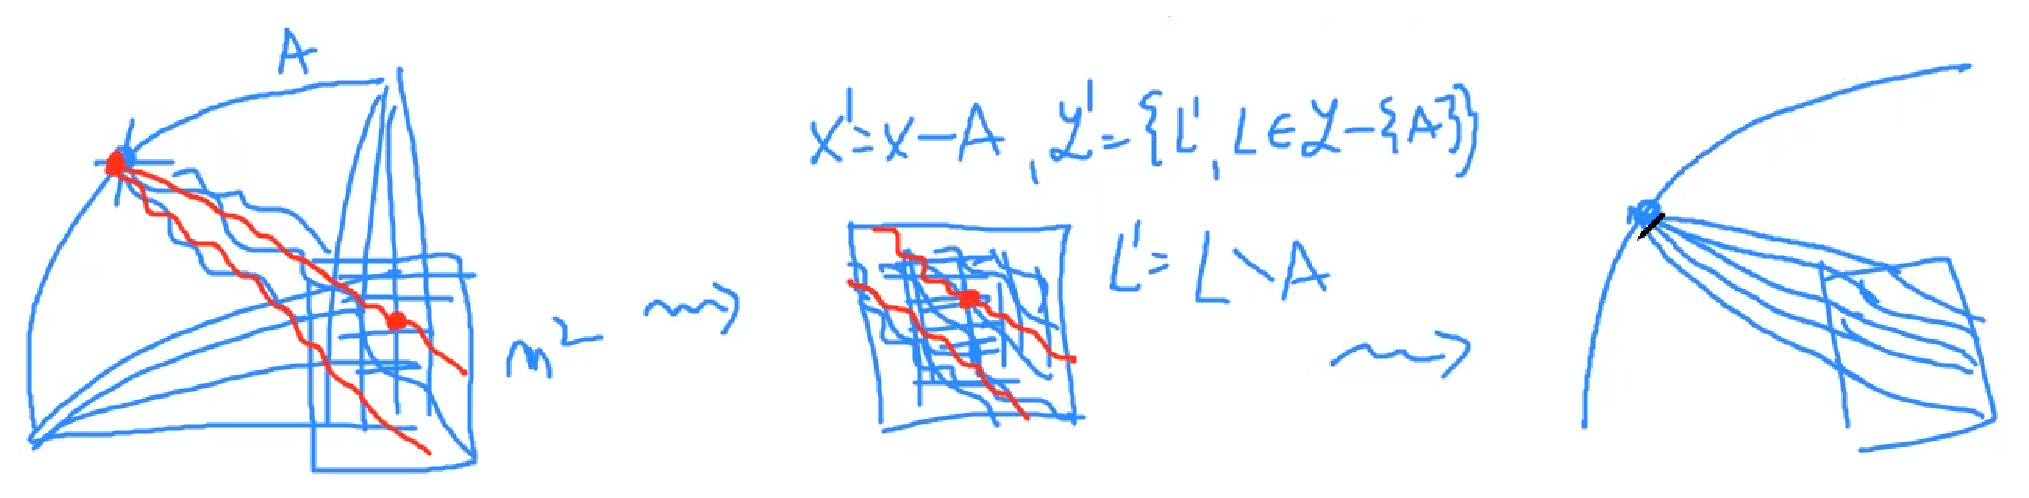
\includegraphics[scale=0.4]{kar_kpr.eps}
\end{consequence}
\begin{definition}[Desargova vlastnost]
    Desargova vlastnost je následující: \emph{Pro každých šest různých bodů $A_1, A_2, B_1,$ $B_2, C_1, C_2$ takových, že se přímky $A_1A_2, B_1B_2, C_1C_2$ protínají v jednom bodě platí, že průsečíky dvojic přímek $A_1B_1, A_2B_2$ a $B_1C_1, B_2C_2$ a $A_1C_1, A_2C_2$ leží na jedné přímce.}
\end{definition}
\begin{definition}[Desargovská projektivní rovina]
    Projektivní rovina je Desargovská, pokud má Desargovu vlastnost. Jinak je ne-Desargovská.
\end{definition}
\begin{exercise}
    KPR sestrojené výše jsou Desargovské.
\end{exercise}

\subsection{KPR a extremální grafy}

% 1 predn 01:08:10
\begin{example}[Extremální Moorovy grafy]
\end{example}

\begin{example}[Copnumber grafu]
\end{example}
